% !TEX program = pdflatex
% PSI-Lens - NASA International Space Apps Challenge 2026
% Strictly 7 frames total (compliant with the 7-slide Global Judging limit).

\documentclass[aspectratio=169,11pt]{beamer}

\usepackage[utf8]{inputenc}
\usepackage[T1]{fontenc}
\usepackage{lmodern}
\usepackage{microtype}
\usepackage{graphicx}
\usepackage{xcolor}
\usepackage{tikz}
\usepackage{booktabs}
\usepackage{hyperref}

\usetikzlibrary{positioning,shapes.geometric,arrows.meta,calc}

% -------------------------------------------------------------------------
% Team & Event Configuration (edit \TeamName here if registered differently)
% -------------------------------------------------------------------------
\newcommand{\TeamName}{Team PSI-Lens}
\newcommand{\EventName}{NASA International Space Apps Challenge 2026}
\newcommand{\ChallengeTitle}{Flame in Freefall: SI-Powered Fire Safety Insights from Microgravity Combustion Data}
\newcommand{\ChallengeURL}{https://www.spaceappschallenge.org/2026/challenges/flame-in-freefall/}
\newcommand{\ReferenceVideoURL}{https://www.youtube.com/watch?v=AVuEiKxOpc0}

% -------------------------------------------------------------------------
% Aerospace Mission-Control Theme Palette
% -------------------------------------------------------------------------
\definecolor{SpaceBg}{HTML}{060B14}
\definecolor{CardBg}{HTML}{0D1729}
\definecolor{CardBgAlt}{HTML}{111E33}
\definecolor{BorderCyan}{HTML}{1E4B63}
\definecolor{BorderOrange}{HTML}{6B3E1D}
\definecolor{AccentCyan}{HTML}{22D3EE}
\definecolor{AccentOrange}{HTML}{FB923C}
\definecolor{AccentGreen}{HTML}{34D399}
\definecolor{TextWhite}{HTML}{F8FAFC}
\definecolor{TextMuted}{HTML}{CBD5E1}
\definecolor{TextDim}{HTML}{94A3B8}

\setbeamercolor{background canvas}{bg=SpaceBg}
\setbeamercolor{normal text}{fg=TextWhite,bg=SpaceBg}
\setbeamercolor{frametitle}{fg=TextWhite}
\setbeamercolor{title}{fg=TextWhite}
\setbeamercolor{itemize item}{fg=AccentCyan}
\setbeamercolor{itemize subitem}{fg=AccentOrange}

\setbeamertemplate{navigation symbols}{}
\setbeamertemplate{itemize item}{\raise0.15ex\hbox{\textcolor{AccentCyan}{\footnotesize$\blacktriangleright$}}}

\hypersetup{
  colorlinks=true,
  urlcolor=AccentCyan,
  linkcolor=AccentCyan,
  pdftitle={PSI-Lens - Space Apps 2026 Demo},
  pdfauthor={Team PSI-Lens}
}

% Clean header and compact 7-slide counter footer
\setbeamertemplate{frametitle}{%
  \vspace*{0.28cm}
  \begin{beamercolorbox}[wd=\paperwidth,leftskip=0.55cm,rightskip=0.55cm]{frametitle}
    \usebeamerfont{frametitle}\textbf{\insertframetitle}\\[-0.18em]
    {\small\color{TextDim}\insertframesubtitle}
  \end{beamercolorbox}
  \vspace*{-0.15cm}
  {\color{BorderCyan}\rule{\paperwidth}{0.5pt}}
}

\setbeamertemplate{footline}{%
  \begin{beamercolorbox}[wd=\paperwidth,ht=0.55cm,dp=0.2cm,leftskip=0.55cm,rightskip=0.55cm]{normal text}
    {\scriptsize\color{TextDim}
      \textbf{\textcolor{AccentCyan}{PSI-LENS}} \textbar{} \TeamName{} \textbar{} \EventName{}
      \hfill
      Slide \textbf{\textcolor{TextWhite}{\insertframenumber}} / \textbf{7}
    }
  \end{beamercolorbox}
}

% Helper styles for dark aerospace cards
\newcommand{\PillCyan}[1]{%
  \tikz[baseline=(X.base)] \node[draw=BorderCyan,fill=CardBgAlt,rounded corners=3pt,inner xsep=6pt,inner ysep=2.5pt,text=AccentCyan,font=\scriptsize\bfseries] (X) {#1};%
}
\newcommand{\PillOrange}[1]{%
  \tikz[baseline=(X.base)] \node[draw=BorderOrange,fill=CardBgAlt,rounded corners=3pt,inner xsep=6pt,inner ysep=2.5pt,text=AccentOrange,font=\scriptsize\bfseries] (X) {#1};%
}
\newcommand{\PillGreen}[1]{%
  \tikz[baseline=(X.base)] \node[draw=AccentGreen!50!SpaceBg,fill=CardBgAlt,rounded corners=3pt,inner xsep=6pt,inner ysep=2.5pt,text=AccentGreen,font=\scriptsize\bfseries] (X) {#1};%
}

\newcommand{\ScreenshotBox}[2]{%
  \begin{tikzpicture}
    \node[draw=BorderCyan,line width=0.9pt,fill=CardBg,rounded corners=5pt,inner sep=3pt] {%
      \includegraphics[width=#1,keepaspectratio]{#2}%
    };
  \end{tikzpicture}%
}

\begin{document}

% =========================================================================
% SLIDE 1 / 7: TITLE, CHALLENGE & PROJECT PREVIEW
% =========================================================================
\begin{frame}[plain]
  \vspace*{0.25cm}
  \begin{columns}[T,onlytextwidth]
    \begin{column}{0.48\textwidth}
      \PillCyan{\EventName}

      \vspace{0.32cm}
      {\fontsize{30}{33}\selectfont\textbf{\textcolor{TextWhite}{PSI-\textcolor{AccentCyan}{Lens}}}}

      \vspace{0.12cm}
      {\large\textbf{\textcolor{TextMuted}{Mission Control for Microgravity Fire Safety}}}

      \vspace{0.35cm}
      
\begin{tikzpicture}
        \node[draw=BorderOrange,line width=0.8pt,fill=CardBg,rounded corners=5pt,inner sep=8pt,text width=\dimexpr\linewidth-18pt\relax,align=left] {%
          {\scriptsize\bfseries\textcolor{AccentOrange}{SELECTED CHALLENGE}}\\[2pt]
          {\small\textbf{\textcolor{TextWhite}{\ChallengeTitle}}}
        };
      \end{tikzpicture}

      \vspace{0.32cm}
      \PillCyan{358 Curated Runs}\hspace{0.12cm}
      \PillOrange{6 NASA Missions}\hspace{0.12cm}
      \PillGreen{AI + Physical Filters}

      \vspace{0.38cm}
      {\scriptsize\bfseries\textcolor{AccentCyan}{TEAM: \TeamName}}\\[3pt]
      {\small\textcolor{TextWhite}{%
        Marcel Bieżuński \textperiodcentered{} Mateusz Frąckowiak \textperiodcentered{} Jakub Grabowski\\
        Jakub Więcław \textperiodcentered{} Bartosz Żelek
      }}
    \end{column}

    \begin{column}{0.50\textwidth}
      \vspace{0.1cm}
      \begin{center}
        \ScreenshotBox{\linewidth}{images/02_explorer_top.png}\\[4pt]
        {\scriptsize\color{TextDim}PSI-Lens Mission Control: natural-language search, SAFFIRE-III overview, and atmosphere map.}
      \end{center}
    \end{column}
  \end{columns}
\end{frame}

% =========================================================================
% SLIDE 2 / 7: WHY IT MATTERS (FOR NON-TECHNICAL JUDGES)
% =========================================================================
\begin{frame}{Why Fire in Space Breaks Every Earth Rule}{From scattered NASA archives to clear insights for students, engineers, and researchers}
  \vspace{0.15cm}
  \begin{columns}[T,onlytextwidth]
    \begin{column}{0.47\textwidth}
      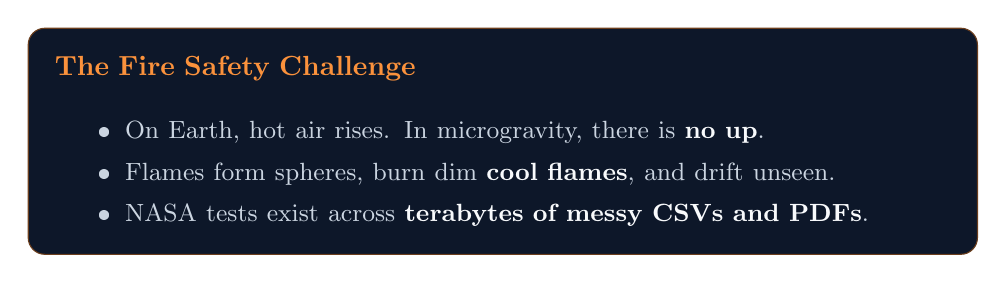
\begin{tikzpicture}
        \node[draw=BorderOrange,fill=CardBg,rounded corners=6pt,inner sep=10pt,text width=\dimexpr\linewidth-22pt\relax] {%
          {\normalsize\textbf{\textcolor{AccentOrange}{The Fire Safety Challenge}}}\\[6pt]
          \small\color{TextMuted}
          \begin{itemize}
            \item On Earth, hot air rises. In microgravity, there is \textbf{\textcolor{TextWhite}{no up}}.
            \item Flames form spheres, burn dim \textbf{\textcolor{TextWhite}{cool flames}}, and drift unseen.
            \item NASA tests exist across \textbf{\textcolor{TextWhite}{terabytes of messy CSVs and PDFs}}.
          \end{itemize}
        };
      \end{tikzpicture}

      \vspace{0.25cm}
      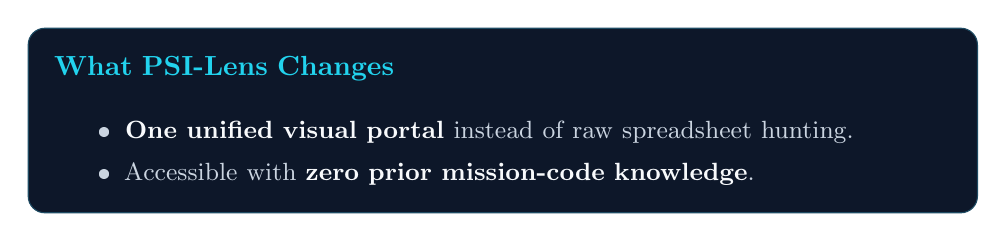
\begin{tikzpicture}
        \node[draw=BorderCyan,fill=CardBg,rounded corners=6pt,inner sep=10pt,text width=\dimexpr\linewidth-22pt\relax] {%
          {\normalsize\textbf{\textcolor{AccentCyan}{What PSI-Lens Changes}}}\\[6pt]
          \small\color{TextMuted}
          \begin{itemize}
            \item \textbf{\textcolor{TextWhite}{One unified visual portal}} instead of raw spreadsheet hunting.
            \item Accessible with \textbf{\textcolor{TextWhite}{zero prior mission-code knowledge}}.
          \end{itemize}
        };
      \end{tikzpicture}
    \end{column}

    \begin{column}{0.50\textwidth}
      \begin{center}
        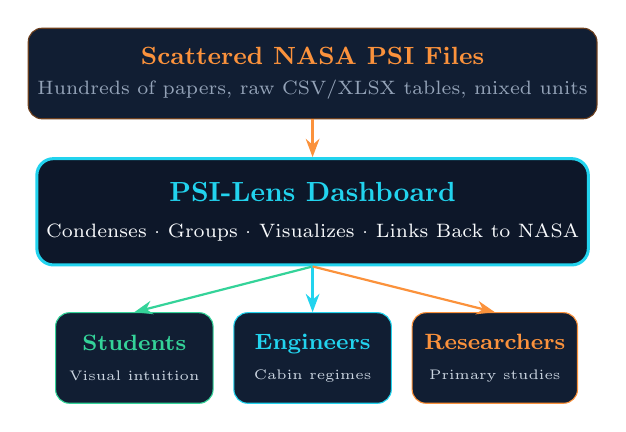
\begin{tikzpicture}[node distance=0.48cm, >=Stealth]
          \node[draw=BorderOrange,fill=CardBgAlt,rounded corners=5pt,minimum width=6.6cm,minimum height=1.15cm,align=center] (raw) {%
            {\small\textbf{\textcolor{AccentOrange}{Scattered NASA PSI Files}}}\\[-1pt]
            {\scriptsize\textcolor{TextDim}{Hundreds of papers, raw CSV/XLSX tables, mixed units}}
          };
          \node[draw=AccentCyan,line width=1.1pt,fill=CardBg,rounded corners=6pt,minimum width=6.6cm,minimum height=1.35cm,align=center,below=of raw] (lens) {%
            {\normalsize\textbf{\textcolor{AccentCyan}{PSI-Lens Dashboard}}}\\[1pt]
            {\scriptsize\textcolor{TextWhite}{Condenses \textperiodcentered{} Groups \textperiodcentered{} Visualizes \textperiodcentered{} Links Back to NASA}}
          };
          \node[draw=AccentCyan,fill=CardBgAlt,rounded corners=5pt,minimum width=2.0cm,minimum height=1.15cm,align=center,below=0.58cm of lens] (eng) {%
            {\footnotesize\textbf{\textcolor{AccentCyan}{Engineers}}}\\[-1pt]
            {\tiny\textcolor{TextMuted}{Cabin regimes}}
          };
          \node[draw=AccentGreen,fill=CardBgAlt,rounded corners=5pt,minimum width=2.0cm,minimum height=1.15cm,align=center,left=0.25cm of eng] (stu) {%
            {\footnotesize\textbf{\textcolor{AccentGreen}{Students}}}\\[-1pt]
            {\tiny\textcolor{TextMuted}{Visual intuition}}
          };
          \node[draw=AccentOrange,fill=CardBgAlt,rounded corners=5pt,minimum width=2.1cm,minimum height=1.15cm,align=center,right=0.25cm of eng] (res) {%
            {\footnotesize\textbf{\textcolor{AccentOrange}{Researchers}}}\\[-1pt]
            {\tiny\textcolor{TextMuted}{Primary studies}}
          };

          \draw[->,thick,AccentOrange] (raw.south) -- (lens.north);
          \draw[->,thick,AccentGreen] (lens.south) -- (stu.north);
          \draw[->,thick,AccentCyan] (lens.south) -- (eng.north);
          \draw[->,thick,AccentOrange] (lens.south) -- (res.north);
        \end{tikzpicture}
      \end{center}
    \end{column}
  \end{columns}
\end{frame}

% =========================================================================
% SLIDE 3 / 7: USER EXPERIENCE - ASK, FILTER, EXPLORE
% =========================================================================
\begin{frame}{User Experience: Ask in Plain English, Explore Live}{AI-assisted hypothesis filtering synchronized with transparent manual controls}
  \vspace{0.1cm}
  \begin{columns}[T,onlytextwidth]
    \begin{column}{0.37\textwidth}
      
\begin{tikzpicture}
        \node[draw=BorderCyan,fill=CardBg,rounded corners=6pt,inner sep=9pt,text width=\dimexpr\linewidth-20pt\relax] {%
          {\small\textbf{\textcolor{AccentCyan}{1. Describe Any Scenario}}}\\[3pt]
          {\footnotesize\color{TextMuted}Type plain English such as \textit{"low cabin pressure"} or click a habitat preset.}
        };
      \end{tikzpicture}

      \vspace{0.2cm}
      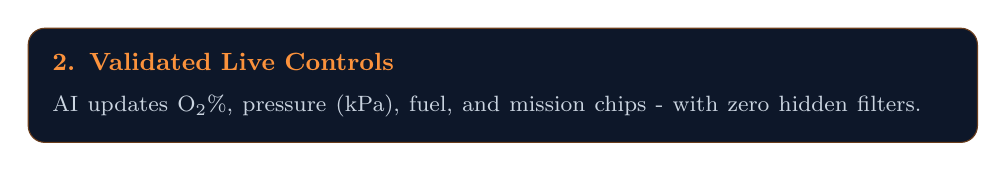
\begin{tikzpicture}
        \node[draw=BorderOrange,fill=CardBg,rounded corners=6pt,inner sep=9pt,text width=\dimexpr\linewidth-20pt\relax] {%
          {\small\textbf{\textcolor{AccentOrange}{2. Validated Live Controls}}}\\[3pt]
          {\footnotesize\color{TextMuted}AI updates O\textsubscript{2}\%, pressure (kPa), fuel, and mission chips - with zero hidden filters.}
        };
      \end{tikzpicture}

      \vspace{0.2cm}
      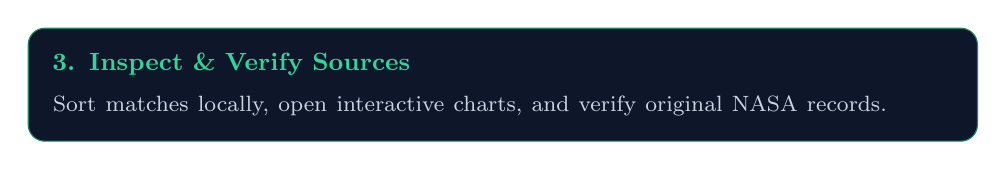
\begin{tikzpicture}
        \node[draw=AccentGreen!60!SpaceBg,fill=CardBg,rounded corners=6pt,inner sep=9pt,text width=\dimexpr\linewidth-20pt\relax] {%
          {\small\textbf{\textcolor{AccentGreen}{3. Inspect \& Verify Sources}}}\\[3pt]
          {\footnotesize\color{TextMuted}Sort matches locally, open interactive charts, and verify original NASA records.}
        };
      \end{tikzpicture}
    \end{column}

    \begin{column}{0.61\textwidth}
      \begin{center}
        \ScreenshotBox{\linewidth}{images/02_scenario_filters.png}\\[3pt]
        {\scriptsize\color{TextDim}Active filter chips, live heat-map bin counts, and filtered run table update together.}
      \end{center}
    \end{column}
  \end{columns}
\end{frame}

% =========================================================================
% SLIDE 4 / 7: NASA OPEN DATA & SPACE TECHNOLOGY
% =========================================================================
\begin{frame}{Powered by NASA Open Data \& Space Technology}{358 verified combustion runs from ISS and Cygnus OA-7 normalized into live JSON}
  \vspace{0.1cm}
  {\scriptsize
  \begin{tabular}{@{}p{2.1cm}p{4.8cm}p{7.2cm}@{}}
    \toprule
    \textbf{\textcolor{AccentCyan}{NASA PSI ID}} & \textbf{\textcolor{TextWhite}{Investigation \& Space Platform}} & \textbf{\textcolor{AccentOrange}{Measured Science Focus}} \\
    \midrule
    \textcolor{AccentCyan}{\textbf{PSI-159}} & ACME CFI-G (ISS \textperiodcentered{} CIR) & Gaseous cool diffusion flames, radiometers, PMT \\
    \textcolor{AccentCyan}{\textbf{PSI-39}}  & CFI / FLEX (ISS \textperiodcentered{} MDCA / CIR) & $D^2$ droplet decay and cool-flame extinction \\
    \textcolor{AccentCyan}{\textbf{PSI-10}}  & ACME Flame Design (ISS \textperiodcentered{} ACME / CIR) & Spherical flame soot-inception \& dilution limits \\
    \textcolor{AccentOrange}{\textbf{PSI-100}} & \textbf{SAFFIRE-III (Cygnus OA-7)} & \textbf{Large 0.4$\times$0.94 m spacecraft fire (30 Hz + 1 Hz)} \\
    \textcolor{AccentCyan}{\textbf{PSI-22}}  & ACME E-FIELD (ISS \textperiodcentered{} ACME / CIR) & Flame response under applied electric fields \\
    \textcolor{AccentCyan}{\textbf{PSI-101}} & SAME-R (ISS \textperiodcentered{} NTRS / PSI) & Microgravity smoke aerosol sizing \& transport \\
    \bottomrule
  \end{tabular}
  }

  \vspace{0.35cm}
  \begin{center}
    
\begin{tikzpicture}[>=Stealth]
      \node[draw=BorderCyan,fill=CardBgAlt,rounded corners=4pt,minimum width=3.1cm,minimum height=0.85cm,align=center] (a) {\scriptsize\textbf{\textcolor{TextWhite}{NASA PSI Data}}\\[-1pt]\tiny\textcolor{TextDim}{Open CSV, XLSX, PDF}};
      \node[draw=BorderCyan,fill=CardBgAlt,rounded corners=4pt,minimum width=3.2cm,minimum height=0.85cm,align=center,right=0.6cm of a] (b) {\scriptsize\textbf{\textcolor{AccentCyan}{Parquet + Polars}}\\[-1pt]\tiny\textcolor{TextDim}{Offline unit normalization}};
      \node[draw=BorderOrange,fill=CardBgAlt,rounded corners=4pt,minimum width=3.1cm,minimum height=0.85cm,align=center,right=0.6cm of b] (c) {\scriptsize\textbf{\textcolor{AccentOrange}{FastAPI + AI}}\\[-1pt]\tiny\textcolor{TextDim}{Validated JSON bounds}};
      \node[draw=AccentGreen,fill=CardBgAlt,rounded corners=4pt,minimum width=3.1cm,minimum height=0.85cm,align=center,right=0.6cm of c] (d) {\scriptsize\textbf{\textcolor{AccentGreen}{React + ECharts}}\\[-1pt]\tiny\textcolor{TextDim}{Null-safe telemetry UI}};
      \draw[->,thick,AccentCyan] (a) -- (b);
      \draw[->,thick,AccentOrange] (b) -- (c);
      \draw[->,thick,AccentGreen] (c) -- (d);
    \end{tikzpicture}
  \end{center}
\end{frame}

% =========================================================================
% SLIDE 5 / 7: SPACECRAFT FIRE TELEMETRY IN ACTION (SAFFIRE-III)
% =========================================================================
\begin{frame}{In Action: Real Spacecraft Fire Telemetry (SAFFIRE-III)}{Synchronizing 30 Hz chamber thermocouples, heat flux, O\textsubscript{2}, and Cygnus downlink}
  \vspace{0.08cm}
  \begin{columns}[T,onlytextwidth]
    \begin{column}{0.66\textwidth}
      \begin{center}
        \ScreenshotBox{\linewidth}{images/01_saffire_top.png}
      \end{center}
    \end{column}

    \begin{column}{0.32\textwidth}
      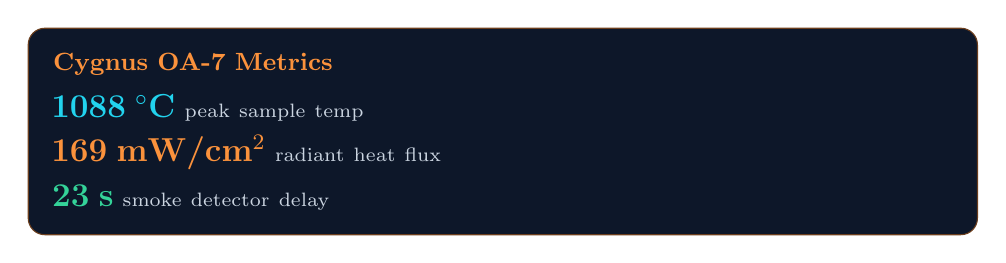
\begin{tikzpicture}
        \node[draw=BorderOrange,fill=CardBg,rounded corners=6pt,inner sep=9pt,text width=\dimexpr\linewidth-20pt\relax] {%
          {\small\textbf{\textcolor{AccentOrange}{Cygnus OA-7 Metrics}}}\\[5pt]
          {\large\textbf{\textcolor{AccentCyan}{1088 $^\circ$C}}} {\scriptsize\textcolor{TextMuted}{peak sample temp}}\\[4pt]
          {\large\textbf{\textcolor{AccentOrange}{169 mW/cm$^2$}}} {\scriptsize\textcolor{TextMuted}{radiant heat flux}}\\[4pt]
          {\large\textbf{\textcolor{AccentGreen}{23 s}}} {\scriptsize\textcolor{TextMuted}{smoke detector delay}}
        };
      \end{tikzpicture}

      \vspace{0.25cm}
      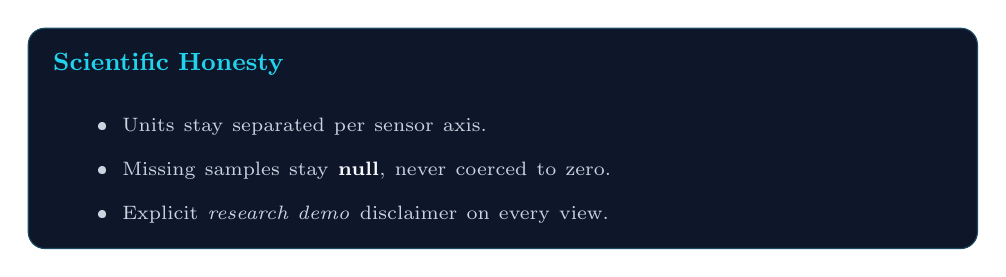
\begin{tikzpicture}
        \node[draw=BorderCyan,fill=CardBg,rounded corners=6pt,inner sep=9pt,text width=\dimexpr\linewidth-20pt\relax] {%
          {\small\textbf{\textcolor{AccentCyan}{Scientific Honesty}}}\\[4pt]
          \scriptsize\color{TextMuted}
          \begin{itemize}
            \item Units stay separated per sensor axis.
            \item Missing samples stay \textbf{\textcolor{TextWhite}{null}}, never coerced to zero.
            \item Explicit \textit{research demo} disclaimer on every view.
          \end{itemize}
        };
      \end{tikzpicture}
    \end{column}
  \end{columns}
\end{frame}

% =========================================================================
% SLIDE 6 / 7: REGIMES & CROSS-RUN COMPARISON
% =========================================================================
\begin{frame}{Safe Exploration: Regimes \& Cross-Run Comparison}{Mapping real O\textsubscript{2} vs. pressure test coverage and aligning runs to ignition}
  \vspace{0.08cm}
  \begin{columns}[T,onlytextwidth]
    \begin{column}{0.49\textwidth}
      \begin{center}
        \ScreenshotBox{\linewidth}{images/03_regime_analytics.png}\\[4pt]
        {\small\textbf{\textcolor{AccentCyan}{Condition Galaxy \& Habitat Regimes}}}\\[2pt]
        {\scriptsize\color{TextMuted}See all 358 measured conditions and nearest same-mission neighbors without inventing unmeasured safety bounds.}
      \end{center}
    \end{column}

    \begin{column}{0.49\textwidth}
      \begin{center}
        \ScreenshotBox{\linewidth}{images/04_cross_run_comparison.png}\\[4pt]
        {\small\textbf{\textcolor{AccentOrange}{Multi-Run Flame Spread Comparison}}}\\[2pt]
        {\scriptsize\color{TextMuted}Pin compatible tests side by side, aligned to verified ignition time ($\Delta t$) with synchronized crosshair inspection.}
      \end{center}
    \end{column}
  \end{columns}
\end{frame}

% =========================================================================
% SLIDE 7 / 7: IMPACT, TEAM & CHALLENGE REFERENCES
% =========================================================================
\begin{frame}{Impact, Team \& NASA Space Apps 2026}{Making microgravity combustion science immediately accessible to everyone}
  \vspace{0.12cm}
  \begin{columns}[T,onlytextwidth]
    \begin{column}{0.48\textwidth}
      
\begin{tikzpicture}
        \node[draw=BorderCyan,fill=CardBg,rounded corners=6pt,inner sep=10pt,text width=\dimexpr\linewidth-22pt\relax] {%
          {\small\textbf{\textcolor{AccentCyan}{PROJECT SUMMARY}}}\\[5pt]
          \footnotesize\color{TextMuted}
          \begin{itemize}
            \item \textbf{\textcolor{TextWhite}{Students:}} Understand zero-g fire intuitively.
            \item \textbf{\textcolor{TextWhite}{Engineers:}} Compare O\textsubscript{2}/pressure \& spacecraft telemetry.
            \item \textbf{\textcolor{TextWhite}{Researchers:}} Trace every chart back to NASA PSI.
          \end{itemize}
        };
      \end{tikzpicture}

      \vspace{0.22cm}
      \begin{tikzpicture}
        \node[draw=BorderOrange,fill=CardBg,rounded corners=6pt,inner sep=10pt,text width=\dimexpr\linewidth-22pt\relax] {%
          {\small\textbf{\textcolor{AccentOrange}{TEAM: \TeamName}}}\\[4pt]
          {\small\textbf{\textcolor{TextWhite}{Team Members:}}}\\[2pt]
          {\footnotesize\color{TextMuted}
            Marcel Bieżuński \textperiodcentered{} Mateusz Frąckowiak \textperiodcentered{} Jakub Grabowski\\
            Jakub Więcław \textperiodcentered{} Bartosz Żelek
          }
        };
      \end{tikzpicture}
    \end{column}

    \begin{column}{0.50\textwidth}
      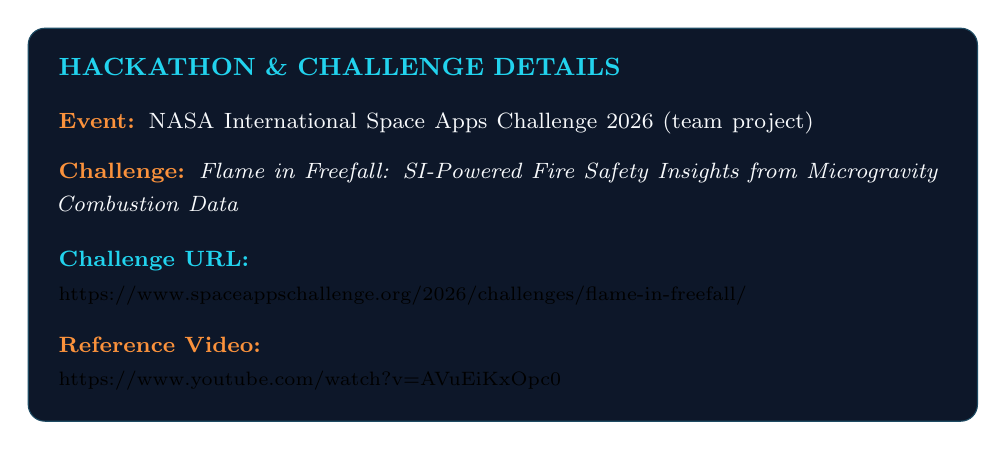
\begin{tikzpicture}
        \node[draw=BorderCyan,fill=CardBg,rounded corners=6pt,inner sep=11pt,text width=\dimexpr\linewidth-24pt\relax] {%
          {\small\textbf{\textcolor{AccentCyan}{HACKATHON \& CHALLENGE DETAILS}}}\\[7pt]
          {\footnotesize\textbf{\textcolor{AccentOrange}{Event:}} \textcolor{TextWhite}{\EventName{} (team project)}}\\[6pt]
          {\footnotesize\textbf{\textcolor{AccentOrange}{Challenge:}} \textit{\textcolor{TextWhite}{\ChallengeTitle}}}\\[8pt]
          {\footnotesize\textbf{\textcolor{AccentCyan}{Challenge URL:}}}\\
          {\scriptsize\url{\ChallengeURL}}\\[7pt]
          {\footnotesize\textbf{\textcolor{AccentOrange}{Reference Video:}}}\\
          {\scriptsize\url{\ReferenceVideoURL}}
        };
      \end{tikzpicture}

      \vspace{0.25cm}
      \begin{center}
        \PillGreen{Thank You - Ready for Questions \& Live Explorer Demo}
      \end{center}
    \end{column}
  \end{columns}
\end{frame}

\end{document}
